\documentclass{article}
\usepackage[backend=bibtex]{biblatex}
\usepackage[margin=1in]{geometry}
\usepackage{amsmath}
\usepackage{amssymb}

\usepackage{graphicx}
\usepackage[space]{grffile} %for filepaths with spaces

\bibliography{../../reports/references.bib} % the name of your .bib bibliography file, without the file extension

% some helpful math commands I like to define
\newcommand{\vect}[1]{\ensuremath{\mathbf{#1}}}
\newcommand{\mat}[1]{\ensuremath{\mathbf{#1}}}
\newcommand{\transpose}{\ensuremath{\mathsf{T}}}
\newcommand{\of}[1]{\ensuremath{\left(#1\right)}}

\newcommand{\degree}{\ensuremath{^\circ}}

% document information
\title{Sensor characterization \\ \large{Optic flow sensor}}
\author{Tim Woodbury}
\date{\today} % or put in a fixed date (e.g. 12 June 2014) if you want it to stay put

% outline:
% Intro
%	objective
%	importance
%	metrics
% Approach
%	Steady-state/at rest characterization
%	flight characterization, compare to VICON
% Results
%	Steady-state
%	Dynamic flight
% Summary

\begin{document}
\maketitle

\section{Introduction}

An important step for filter design on the quadrotor platforms is characterization of the onboard sensors. The sensor models developed will enable sequential filter design and will influence how data are processed, such as outlier rejection and/or bias compensation. The vehicle inertial measurement unit (IMU) hass been previously characterized by comparing at-rest performance with sensor returns during hovering flight. In this document, an investigation of the optic flow sensor performance is offered. The optic flow sensor only returns meaningful values when the sensor height-above-ground distance is greater than the minimum range of its sonar sensor (approximately 30 cm), so at-rest readings are not relevant. The flow sensor is characterized by flying the vehicle at different altitudes and comparing flow sensor readings with inertial measurements from the Optitrack measurement system.

\section{Approach}

%Special consideration was given to the optic flow sensor. One test was conducted with the vehicle at rest on a cart, approximately 0.9 m above the floor, to examine the zero-velocity flow measurements. A second test was conducted while the cart was moved around, and data were compared against Optitrack inertial measurements. A third test was conducted with the vehicle in position hold mode, flying along the body 1 and 2 axes at different altitudes (limited by the extent to which the vehicle will hold altitude).

\section{Results}

The sensor measurements of interest from the optic flow sensor are the compensated x and y velocities and ultrasonic rangefinder reading. The velocities are provided in the plane defined by the flow camera axis, and the angular rotation of the sensor is accounted for in the provided values. The primary values of interest are the variance of the x and y velocities, the minimum velocity and altitude required for the system to function, and the variance of the ultrasonic sensor.

\subsection{Velocities}

The optic flow sensor has some unusual limitations. The sensor is rated for a maximum flow velocity of 1.5 rad/s \cite{honegger2013} or, more practically, approximately 1 m/s per meter of altitude. It is expected that the sensor performance may vary with altitude, and it should be determined if there is a minimum required speed for the sensor to provide meaningful results. It should be noted that the flow sensor outputs a ``quality'' metric, consisting of a single byte, indicating how good the measurements are. It is assumed that this value is inversely proportional to an internally propagated variance. It is further assumed that readings will not be used when the flow quality metric is low. Based on the observed variance in flight data, the minimum quality threshold is selected as 215 (out of a maximum of 255).

To characterize the sensor, the vehicle is flown under manual control and measurements compared with Optitrack data. Two flights are conducted and compared. The flow measurement histories are manually segmented into regions with visibly low variance, and the mean and standard error of measurement errors in those segments are contrasted with the mean and standard error in the rest of the flight. ``The rest of the flight'' should be interpreted as the flight segments where the flow quality threshold is met or exceeded.

\begin{table}
\centering
\begin{tabular}{c|c|c|c|c|c|c|c|c}
Flight & $\mu(\epsilon_{v_x})$ & $\mu(\epsilon_{v_y})$ & $\sigma(\epsilon_{v_x})$ & $\sigma(\epsilon_{v_y})$ & $\mu(|v_x|)$ & $\mu(|v_y|)$ & $\mu(h)$ & length (sec)\\
1, manual segments & .0029 & .011 & .66 & .59 & 0.20 & 0.18 & 1.1 & 32.5\\
1, $Q > 215$ & .077 & -.056 & 0.88 & 0.82 & 0.43 & 0.4 & 1.3 & 70.9\\
2, manual segments & .047 & -.028 & 1.1 & 1.1 & 0.41 & 0.46 & 1.9 & 105 \\
2, $Q > 215$ & .025 & .0051 & 1.1 & 1.1 & 0.5 & 0.56 & 1.6 & 187
\end{tabular}
\caption{Tabulated results from flight tests of flow sensor. ``Manual segments'' refers to those selected as having visibly low flow variance. ``$Q > 215$'' refers to all parts of the flight where the quality value reported exceeds the selected threshold. Residuals for the flow sensor x  and y speeds are indicated by $\epsilon_{v_x}$ and $\epsilon_{v_y}$ respectively and have units of m/s. Residuals are computed with respect to the Optitrack velocities transformed into the flow sensor frame. The mean $\mu$ and standard error $\sigma$ of each residual is reported. Mean altitude in meters from Optitrack is also reported. The length of each data segment is given in seconds for reference.}
\label{tab:flight_data}
\end{table}

Table \ref{tab:flight_data} summarizes findings from the two flights. Data from the segments selected as having apparently lower variance are compared against all segments where the flow quality is sufficiently high. This is done to determine if the flow errors and variance are actually noticeably different. The tabulated data indicate that the mean flow errors are typically of the order of 0.01 m/s. The standard error may be as large as about 1 m/s, and the standard error is larger for segments with a higher mean altitude, suggesting a possible interaction effect. The lowest standard error occurs during the segment with the lowest mean velocities, suggesting another possible interaction.

Based on these findings, an investigation is made into the dependence of the residuals on altitude and on true flow-frame velocity. Errors were binned based on altitude rounded to the nearest 0.125 m, and the variance of each bin was computed. Results are shown in Fig. \ref{fig:resids_v_alt_bins}. A proposed model is also shown. As a function of altitude, $h$, the proposed model gives the standard deviation $\sigma(h)$ for each axis as:

\begin{equation}
\sigma(h) = \begin{cases}
0.4 \ \mathrm{m/s}, & \text{if $h \leq 0.5 $ m} \\
(0.68h + .06) \ \mathrm{m/s}, & \text{if $ .5 < h \leq 1.75 $ m} \\
1.25 \ \mathrm{m/s}, & \text{if $h > 1.75 $ m}
\end{cases}
\label{eq:sigmamodel}
\end{equation}

Figs. \ref{fig:resids_v_alt1}-\ref{fig:resids_v_alt2} show all errors plotted against altitude for the two flights. For reference, the errors in the manually identified low-variance segments are shown. Based on the plots, the proposed fit for $\sigma(h)$ appears to be conservative for the first flight, and reasonably close to the observed error distribution in the second flight. For simulation purposes, Eq. \ref{eq:sigmamodel} is proposed for the optic flow sensor. For estimation purposes, the maximum value of 1.25 m/s is suggested as the sensor standard deviation.

\begin{figure}
\centering
\begin{minipage}{0.49\textwidth}
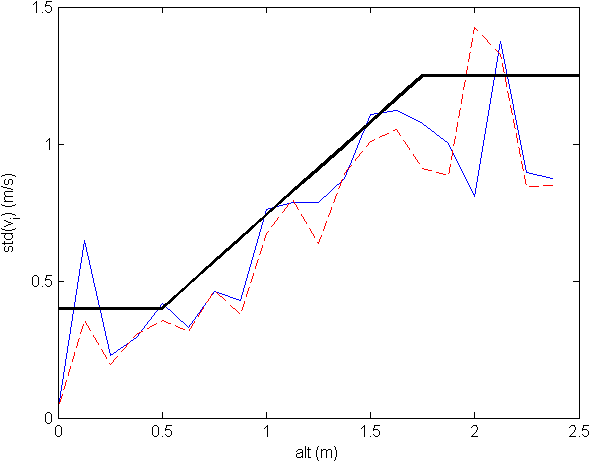
\includegraphics[width=\textwidth]{../flow figures/resids_v_alt1_bins.png}
\end{minipage}
\begin{minipage}{0.49\textwidth}
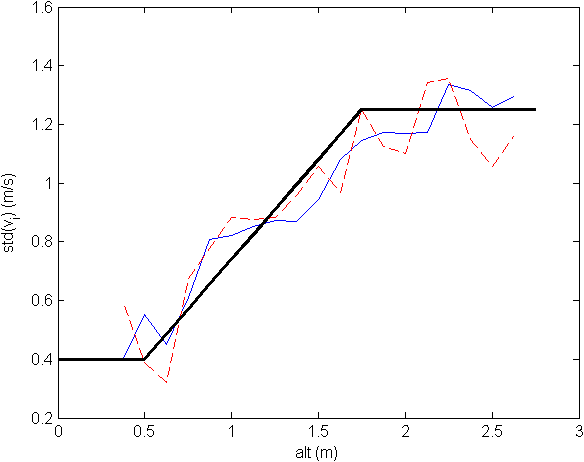
\includegraphics[width=\textwidth]{../flow figures/resids_v_alt2_bins.png}
\end{minipage}
\caption{Variance of binned errors for the two flights. Solid lines indicate the sensor x-axis error, dashed lines indicate the y-axis error. The black line indicates the suggested fit and is the same for both figures.}
\label{fig:resids_v_alt_bins}
\end{figure}

\begin{figure}[p]
\centering
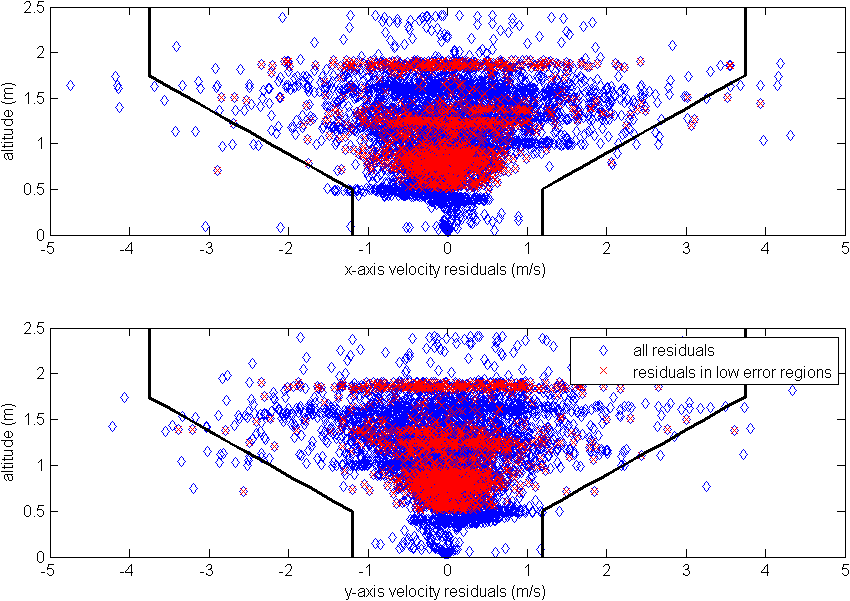
\includegraphics[height=0.4\textheight]{../flow figures/resids_v_alt1_w_3sigma.png}
\caption{X and Y axis errors with proposed $3\sigma$ fit for flight 1.}
\label{fig:resids_v_alt1}
\end{figure}
\begin{figure}[p]
\centering
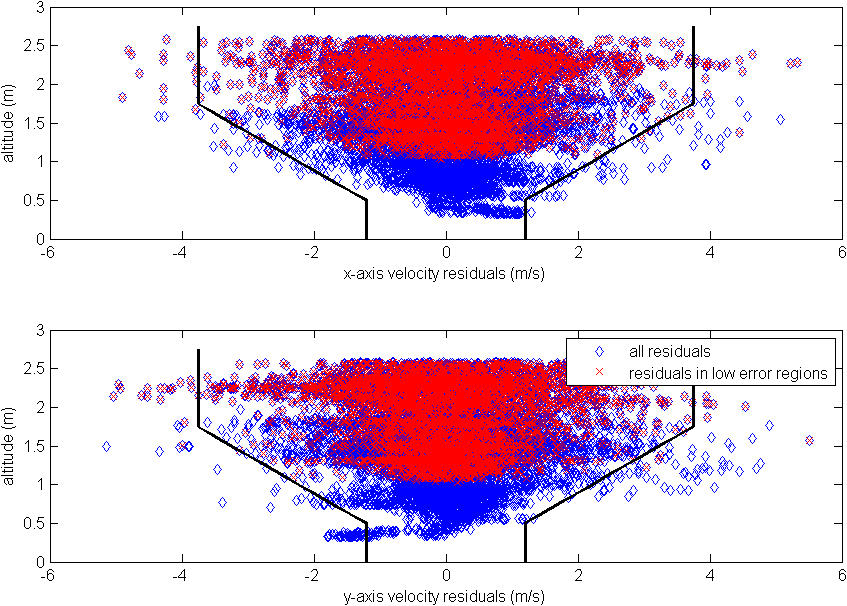
\includegraphics[height=0.4\textheight]{../flow figures/resids_v_alt2_w_3sigma.png}
\caption{X and Y axis errors with proposed $3\sigma$ fit for flight 2.}
\label{fig:resids_v_alt2}
\end{figure}

Figs. \ref{fig:resids_v_vel1}-\ref{fig:resids_v_vel2} plot measurement errors versus Optitrack truth values. These plots contrast the distribution in the selected low-variance regions against the all the sections with high enough quality. In addition, errors when the true velocity is less than 1 m/s per meter of altitude are indicated. For both flights, most of the data points with high quality already meet this criterion, but there are a few outliers. The blue and black data points for all the charts show some suggestion of a one-to-one slope; in a plot of errors versus true value, a one-to-one slope indicates the measurement is 100\% noise, an undesirable feature. The errors in the manually selected regions appear to have a less prominent slope, with the slope being most notable as the true velocity grows larger. In Fig. \ref{fig:resids_v_vel2}, the errors for true velocities of less than 1 m/s are highlighted, and have a yet less visible slope; for the first flight, the red and green data points are indistinguishable and the green are omitted.

Table \ref{tab:velvserr} summarizes the slopes of the residuals as functions of the true velocities. (Note that these values are given in degrees.) The relationship is definitely not one-to-one, but the linear relationship is also much stronger than is ideal. It is noted that the slope is noticeably less in the user-selected regions, and it would be good if these lower-error regions could be predicted from the flow data alone. Unfortunately, a good predictive relationship was not found. When flow velocities of less than 1 m/s were intersected with flow quality readings above 215, the resulting error-velocity slope was roughly 40\degree for both axes. Verifying that flow velocity is less than 1 m/s per meter of measured altitude was somewhat more fruitful, having a slope of roughly 30\degree typically. This value is similar to the slope in regions where the true velocity is less than 1 m/s per meter of true altitude. This check on flow velocity versus measured altitude is the best one found to predict low-noise measurements.

\begin{table}
\centering
\begin{tabular}{c|c|c|c|c}
Flight & $b_{v_x}$ & $b_{v_y}$ & $b_{v_x'}$ & $b_{v_y'}$ \\
1 & 27 & 29 & 17 & 23\\
2 & 21 & 33 & 11 & 15\\
\end{tabular}
\caption{Summary of best-fit slope of the velocity errors as functions of true velocities in each flight. $b_{v_x}$ and $b_{v_y}$ indicate the slope of x-velocity and y-velocity errors versus their respective truth values in meters. $b_{v_x}'$ and $b_{v_y}'$ indicate the slope in the regions indicated by red in Figs. \ref{fig:resids_v_vel1} and \ref{fig:resids_v_vel2}; that it, the intersection of regions manually selected as having low variance and regions where the true velocity is less than 1 m/s per meter of altitude.}
\label{tab:velvserr}
\end{table}

\begin{figure}[p]
\centering
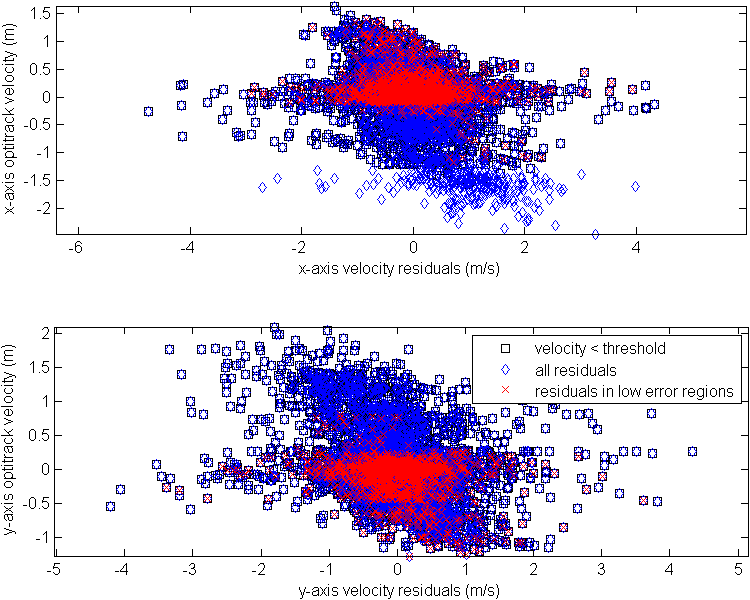
\includegraphics[height=0.4\textheight]{../flow figures/resids_v_vel.png}
\caption{X and Y axis errors versus Optitrack velocities for flight 1.}
\label{fig:resids_v_vel1}
\end{figure}
\begin{figure}[p]
\centering
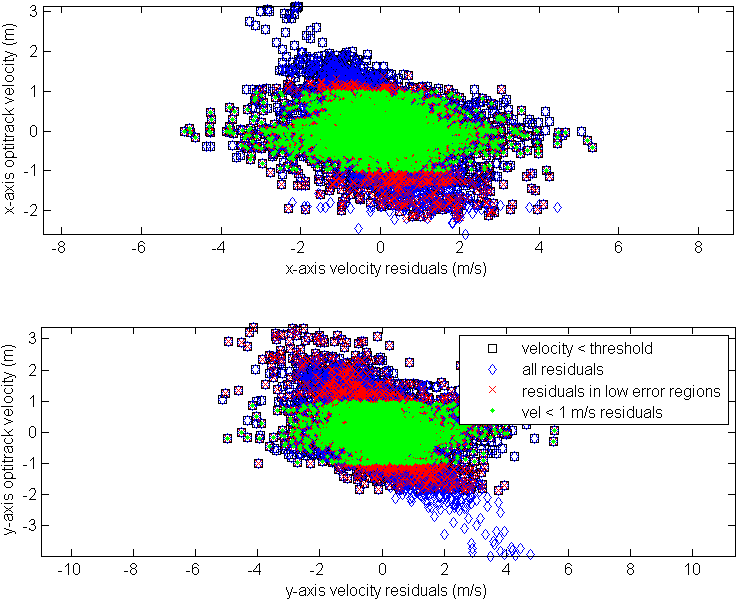
\includegraphics[height=0.4\textheight]{../flow figures/resids_v_vel2.png}
\caption{X and Y axis errors versus Optitrack velocities for flight 2.}
\label{fig:resids_v_vel2}
\end{figure}

\subsection{Sonar}

The ultrasonic rangefinder is a component of the optic flow sensor board. The rangefinder is characterized by comparing sensor returns against Optitrack position measurements. (This admits some error by neglecting consideration of attitude effects on the rangefinder outputs. Some bias between the center of mass defined in Optitrack and the location of the rangefinder is expected, and should be on the order of centimeters.) Fig. \ref{fig:movingflyingalt} shows typical rangefinder measurements compared to Optitrack data. The measurements match the Optitrack data well except for a notable number of outliers, which are clearly some sort of false returns. The rate of occurrence of these outliers is approximately 10\%, and is quantified in two tests.

Fig. \ref{fig:movingflyingalthist} shows a histogram of altitude errors once outliers are removed. More errors are concentrated near zero than the Gaussian distribution suggests, so this fit should be conservative. Table \ref{tab:altErrs} shows the mean and standard deviation of altitude measurement errors, ignoring outliers, as well as the fraction of samples that are outliers. It can be seen that the fraction of outliers may be quite high, and should be accounted for in data management. The bias is reasonably approximated as less than 5 centimeters typically (this figure includes uncertainty in the Optitrack-rangefinder relative offset). As a conservative bound, 150\% of the maximum of the measured standard deviations is taken as the error bound:

\begin{equation}
\sigma_{alt} = 0.083 \ \mathrm{m}
\end{equation}

\begin{figure}[tb!]
\centering
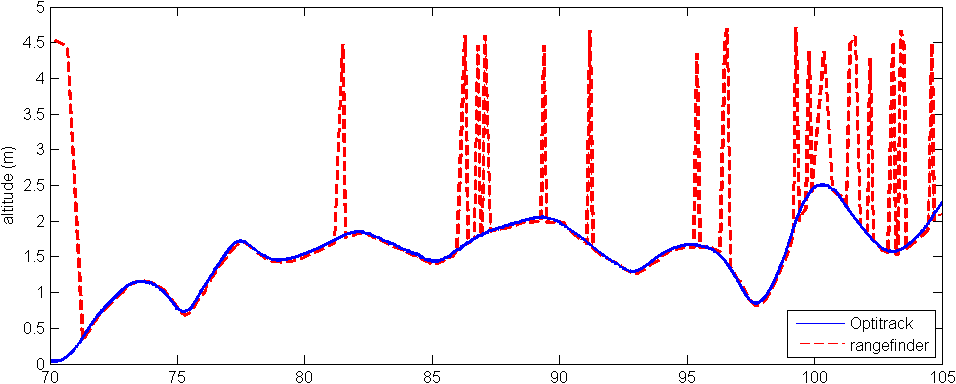
\includegraphics[width=\textwidth]{../moving_flying_alt.png}
\caption{Altitude measurements during flight.}
\label{fig:movingflyingalt}
\end{figure}

\begin{table}
\centering
\begin{tabular}{c|c|c|c}
Segment & Mean altitude error (m) & Error standard deviation (m)& Fraction of bad returns\\
1 & 0.035 & 0.055 & 0.20\\
2 & 0.026 & 0.031 & 0.085\\
\end{tabular}
\caption{Summary of in-flight errors from ultrasonic rangefinder.}
\label{tab:altErrs}
\end{table}

\begin{figure}[tb!]
\centering
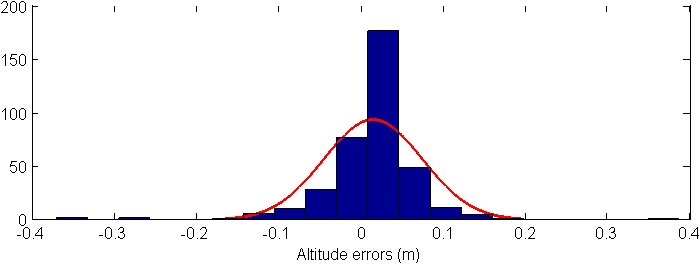
\includegraphics[width=\textwidth]{../moving_flying_alt_hist.png}
\caption{Histogram of ultrasonic rangefinder measurements after outliers are removed..}
\label{fig:movingflyingalthist}
\end{figure}

\section{Summary}

The principle findings with regard to the flow sensor are:

\begin{enumerate}
\item Flow velocity biases are typically on the order of 0.01 m/s.
\item Flow error standard deviation can be conservatively given by Eq. \ref{eq:sigmamodel} as a function of altitude, and by $\sigma = 1.25$ m/s as an upper bound.
\item Flow readings should not be used when the flow quality is below 215.
\item Flow readings should not be used when the measured velocity is greater than 1 m/s per meter of altitude. If velocity and altitude estimates are available, these may be used for possibly greater accuracy in predicting ``bad'' flow measurements.
\end{enumerate}

The findings with regard to the sonar sensor are:

\begin{enumerate}
\item ``True'' sonar measurements have as assumed error standard deviation of 0.083 m.
\item ``False'' sonar measurements occur at a rate of between 8\% and 20\%, based on flight data.
\item Typical sonar bias is on the order of centimeters, and should be covered by an assumed bound of 5 cm.
\end{enumerate}

\printbibliography

\end{document}
